\documentclass[12pt]{article}
\setlength\parindent{0pt}
\usepackage{fullpage}
\usepackage{epsf}
\usepackage{amsmath}
\usepackage{graphicx}
\setlength{\parskip}{4mm}
\def\LL{\left\langle}   % left angle bracket
\def\RR{\right\rangle}  % right angle bracket
\def\LP{\left(}         % left parenthesis
\def\RP{\right)}        % right parenthesis
\def\LB{\left\{}        % left curly bracket
\def\RB{\right\}}       % right curly bracket
\def\PAR#1#2{ {{\partial #1}\over{\partial #2}} }
\def\PARTWO#1#2{ {{\partial^2 #1}\over{\partial #2}^2} }
\def\PARTWOMIX#1#2#3{ {{\partial^2 #1}\over{\partial #2 \partial #3}} }
\newcommand{\BE}{\begin{displaymath}}
\newcommand{\EE}{\end{displaymath}}
\newcommand{\BNE}{\begin{equation}}
\newcommand{\ENE}{\end{equation}}
\newcommand{\BEA}{\begin{eqnarray}}
\newcommand{\EEA}{\nonumber\end{eqnarray}}
\newcommand{\EL}{\nonumber\\}
\newcommand{\la}[1]{\label{#1}}
\newcommand{\ie}{{\em i.e.\ }}
\newcommand{\eg}{{\em e.\,g.\ }}
\newcommand{\cf}{cf.\ }
\newcommand{\etc}{etc.\ }
\newcommand{\Tr}{{\rm tr}}
\newcommand{\etal}{{\it et al.}}
\newcommand{\OL}[1]{\overline{#1}\ } % overline
\newcommand{\OLL}[1]{\overline{\overline{#1}}\ } % double overline
\newcommand{\OON}{\frac{1}{N}} % "one over N"
\newcommand{\OOX}[1]{\frac{1}{#1}} % "one over X"

\pagenumbering{gobble}

\begin{document}


\bigskip
\bigskip
\bigskip
\bigskip

\Large \centerline{\sc{Physics 211 Exam 1 Practice}}


\vspace{2in}

\normalsize

\vspace{1.4in}

\begin{itemize}
\item{This practice exam is in exactly the same format as the real exam will be, but it is more than twice as long.}
\item{The real exam will be either four or five questions.}
\item{On the real exam, you may use any electronic or graphing calculator, but no cellphones, computers, etc.}
  \item{``Graph'' means to make a precise graph on a separate sheet of graph paper. The locations of intercepts, inflection points, maxima and minima, slopes, and the sign of concavity need to be accurate.}
  \item{``Sketch'' means to make a casual graph which does not need to be on a separate page. These sketches need to illustrate only the essential features of the motion; they do not
    need to be perfectly to scale.}
  \item{{\bf You must show your reasoning to receive credit}. A numerical answer with no logic shown will be treated as no answer.}
  \item{Remember, show your reasoning as thoroughly as possible for partial credit.}
  \item{Use $g=10\, \rm m/\rm s^2$ throughout to minimize arithmetic.}
\end{itemize}
\newpage
\small

\begin{flushright}
  Name: \underline{\hspace{3in}}
\end{flushright}



\Large \centerline{\sc{Question 1}}
\normalsize

A bucket hangs from a rope, 10m below the edge of a cliff. This rope is connected to a motor that accelerates it upward at $2 \frac{\rm m}{\rm s^2}$.

\it{a) How long does the bucket take to rise to the cliff edge after the motor is switched on?}

\vspace{1in}

\it{b) What is its speed when it arrives there?}

\vspace{1in}

At the same instant as the motor is switched on, a stone is dropped from the edge of the cliff. (Both objects start from rest.)

\bigskip

\it{c) Sketch the position vs. time of the bucket and of the stone on the same set of axes.}

\vspace{1in}

\it{d) How long after the objects begin moving does the stone land in the bucket?}

\vspace{1in}

\it{e) How far does the stone fall before it lands in the bucket?}

\newpage

\begin{flushright}
    Name: \underline{\hspace{3in}}
  \end{flushright}

  \Large \centerline{\sc{Question 2}}
  \normalsize
\rm

Alice is standing on the street with a baseball. Bob is watching above from a window at a height of 5m above her. She throws the ball straight upward to him at
a speed of 15 $\frac{\rm m}{\rm s}$, and he catches it as it flies upward.

\bigskip

\it{a) How long is the ball in the air before he catches it?}

\vspace{3in}

\it{b) The quadratic formula gives you two roots. One of these will help you answer the preceding question. What is the physical interpretation of the other root?}
\vspace{1in}

\it{c) What is the ball's velocity when he catches it?}


  \newpage

\begin{flushright}
    Name: \underline{\hspace{3in}}
  \end{flushright}

  \Large \centerline{\sc{Question 3}}
  \normalsize
\rm

A hiker on flat ground walks at a constant speed. She walks north for one hour, walks for two hours at an angle $30^o$ south of west, then walks for three hours at an angle
$45^o$ north of east. (In the Cartesian plane: she walks in the positive $y$-direction for one hour, walks for two hours at an angle $30^o$ below the negative $x$-axis, then walks 
for three hours at an angle $45^o$ above the positive $x$-axis.)

Hint: What is a reasonable unit to measure distance in for this problem?

\bigskip
  
\it

a) How long must she walk to return to her starting point?

\vspace{3in}

b) In what direction must she walk to return to her starting point?


\newpage






        \Large \centerline{\sc{Question 4}}
        \normalsize
        \rm

A ball is thrown from ground level at a speed $v_0$ at an angle $\theta$ above the horizontal.

\bigskip

Give your answers to the following in terms of $g$, $v_0$, and $\theta$. If you run out of room, use the back of the page.

\it \bigskip

a) What are the horizontal and vertical components of the ball's initial velocity?

\vspace{1in}

b) What functions $x(t)$ and $y(t)$ give its position as a function of time?

\vspace{1in}

c) How long after it is thrown does the ball land back on the ground? 

\vspace{1in}

d) How far away from the starting point does the ball land? 

\vspace{1in}

e) What is the maximum height achieved by the ball?

\newpage


\begin{flushright}
Name: \underline{\hspace{3in}}
        \end{flushright}

        \Large \centerline{\sc{Question 5}}
        \normalsize
        \rm

A frog jumps horizontally off of a table 2 m high. It lands on the floor 1.5 m away from the bottom of the table.

\it \bigskip

a) How long was the frog in the air? (5 points)

\vspace{1.2in}

b) What initial velocity did the frog jump with? (10 points)

\vspace{1.2in}

c) What are the $x-$ and $y-$components of the frog's velocity when it lands on the ground? (5 points)

\vspace{1.2in}

d) What is the frog's speed when it lands on the ground? (2 points)

\vspace{1in}

e) What is the angle between the frog's velocity vector and the $x$-axis when it lands? (3 points)

\bigskip

\newpage
\begin{flushright}
Name: \underline{\hspace{3in}}
        \end{flushright}

        \Large \centerline{\sc{Question 6}}
        \normalsize
        \rm

The velocity vs. time graph for an object is shown below.

\centerline{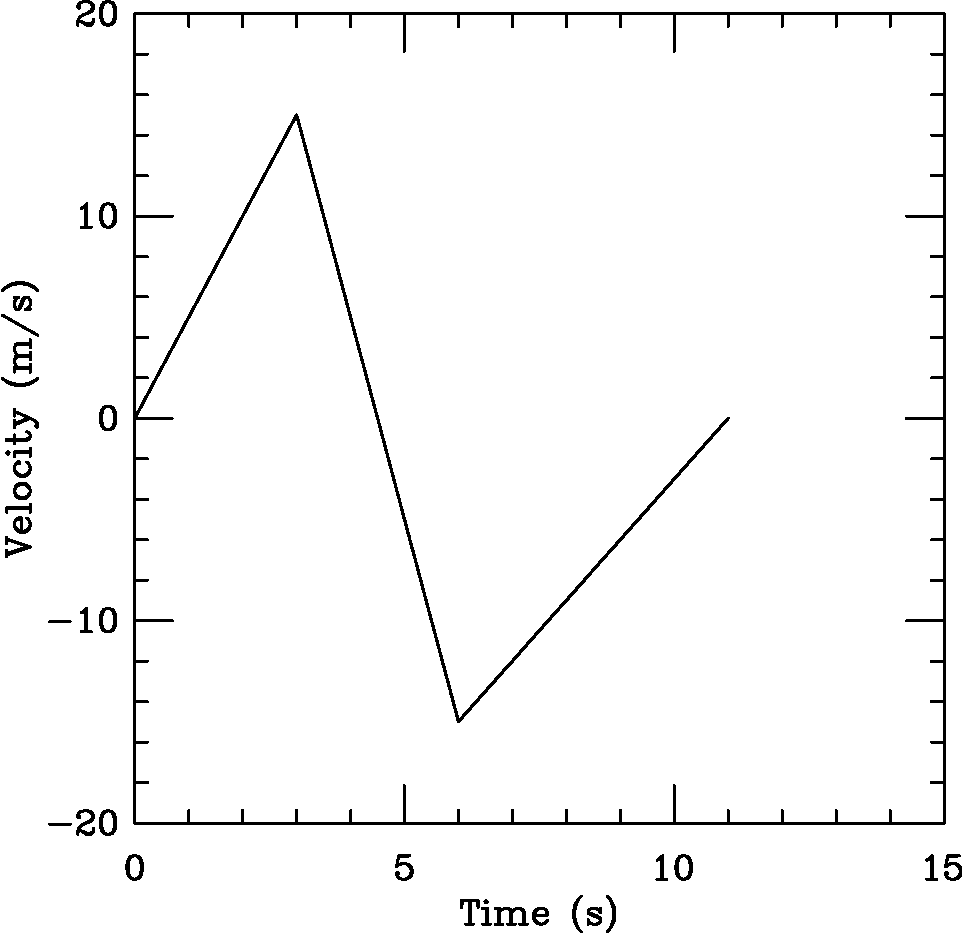
\includegraphics[width=0.4\textwidth]{vel-crop.pdf}}
\it \bigskip

a) Sketch a graph of acceleration vs. time for the object.
\vspace{2.2in}

b) Sketch a graph of position vs. time for the object.


\newpage

\begin{flushright}
Name: \underline{\hspace{3in}}
        \end{flushright}

        \Large \centerline{\sc{Question 7}}
        \normalsize
        \rm

A rocket is dropped out of a window and pointed sideways toward another building. One
second after it is dropped, its motor fires, giving it an acceleration of $2g$ in the horizontal
direction. (Its vertical acceleration is still $g$ downward.)

After the motor fires, the rocket flies along its new path until it strikes another building,
located 40 m away.

\it \bigskip

a) How long (in total) was the rocket in the air?

\vspace{1.5in}


b) How far below the level of the window did the rocket strike the building?

\vspace{1.5in}

c) Graph $v_x$ and $v_y$ as a function of time.

\newpage

\begin{flushright}
Name: \underline{\hspace{3in}}
        \end{flushright}

        \Large \centerline{\sc{Question 8}}
        \normalsize
        \rm

A person throws a heavy ball into the air at a speed of 10 m/s at an angle 30 degrees below the
vertical. This is done in a large room with a ceiling made out of paper; the ceiling’s height is
2m above the level where she released the ball. This ball will punch two holes in the paper
ceiling, one on the way up and one on the way down. 

\it

How far apart are the two holes?


\newpage

\begin{flushright}
Name: \underline{\hspace{3in}}
        \end{flushright}

        \Large \centerline{\sc{Question 9}}
        \normalsize
        \rm

A ball is dropped from a height of 20 m. The ball bounces when it strikes the ground, such
that the ball rebounds at a speed equal to half the speed that it struck the ground with.

\it
a) How long does it take to hit the ground (the first time)?

\vspace{1.5in}

b) How fast is the ball traveling when it strikes the ground?
\vspace{1.5in}

c) How high does the ball bounce?
\vspace{1.5in}

d) Graph the ball's velocity vs. time, starting at the moment the ball is dropped
and continuing to the point where the ball strikes the ground again after it bounces.


\end{document}
